\documentclass[conference]{IEEEtran}
\IEEEoverridecommandlockouts

% The preceding line is only needed to identify funding in the first footnote. If that is unneeded, please comment it out.
\usepackage{cite}
\usepackage{amsmath,amssymb,amsfonts}
\usepackage{algorithmic}
\usepackage{graphicx}
\usepackage{textcomp}
\usepackage{listings}
\usepackage{xcolor}
\def\BibTeX{{\rm B\kern-.05em{\sc i\kern-.025em b}\kern-.08em
    T\kern-.1667em\lower.7ex\hbox{E}\kern-.125emX}}

% -----
\usepackage{fontspec}
\usepackage{xltxtra}
\usepackage{xunicode}
\usepackage{scrextend}

% Thai Language setup
\XeTeXlinebreaklocale{'th'}
\newfontfamily\thaifont{TH Sarabun New}
\setmainfont{TH Sarabun New}
\changefontsizes[12pt]{12pt}
\XeTeXlinebreakskip = 0pt plus 1pt
\defaultfontfeatures{Scale=1.23}
% -----

\def\StudentId{63199130350}
\def\Me{นายสิทธิพงษ์ เหล่าโก้ก}
\def\MyEmail{sitdhibong.laokok@g.swu.ac.th}
\def\SNATopic{พฤติกรรมของผู้เรียนในระบบการเรียนออนไลน์ขนาดใหญ่ซึ่งนำไปสู่การยุติการเรียน}
\def\SNATopicEN{Behavior of Online Learner in MOOC Platform Leading to Course Drop-out}
\def\VirtualClassroom{ห้องเรียนเสมือน}
\def\moocs{การเรียนการสอนขนาดใหญ่}
\def\MOOCs{ระบบ{\moocs}}
\def\dropout{ยุติการเรียนกลางคัน}

% English overwrite
\def\IEEEkeywordsname{คำสำคัญ}
\def\abstractname{บทคัดย่อ}
\def\figurename{รูปที่}
\def\tablename{ตารางที่}

\title{ \SNATopic }
\author{
    \IEEEauthorblockN{\Me} \newline
    \IEEEauthorblockA{\MyEmail} \newline
    \IEEEauthorblockA{ภาคการศึกษาที่ 2 ประจำปีการศึกษา 2563} \newline
    \IEEEauthorblockA{ภาควิชาวิทยาการคอมพิวเตอร์ คณะวิทยาศาสตร์} \newline
    \IEEEauthorblockA{มหาวิทยาลัยศรีนครินทรวิโรฒ ประสานมิตร}
}

% Command
\newcommand*{\thead}[1]{\multicolumn{1}{c}{\bfseries #1}}

\begin{document}

    \maketitle

    \begin{abstract}
        Lorem ipsum
    \end{abstract}

    \begin{IEEEkeywords}
        MOOC, Learner Behavior, Online Course Dropout, Online Course Retired
    \end{IEEEkeywords}

    % = = = = = = = = = = = = = = =
    \section{บทนำ}
    เมื่อเกิดการระบาดของโคโรนาไวรัส (Coronavirus) ในช่วงปลายปี พ.ศ. 2562 \cite{covid:coronavirus}
    ที่แพร่ระบาดไปทั่วโลก และยังคงระบาดอย่างต่อเนื่องอยู่ในหลายประเทศทั่วโลก \cite{covid:worldtrendspread}
    รวมถึงในประเทศไทย \cite{covid:thailandspread} ที่เกิดการแพร่ระบาดเพิ่มมากขึ้นเรื่อยๆ
    ส่งผลให้เกิดมาตรการควบคุมกิจกรรมออกมา เพื่อลดการมีปฏิสัมพันธ์กันระหว่างบุคคล 
    และควบคุมสถานการณ์การระบาดของโคโรนาไวรัส \cite{covid:ratchakitcha:22}
    ทั้งนี้ ส่งผลให้หลายกิจกรรมนั้นจำเป็นต้องปรับเปลี่ยนการดำเนินกิจกรรมจากเดิม
    ให้สอดคล้องกับมาตรการควบคุม และคำแนะนำทางด้านสาธารณสุข \cite{covid:socialdistancing} 
    ทั้งการเพิ่มระยะห่างในการทำกิจกรรม การลดระยะเวลาการให้บริการ 
    ไปจนกระทั่งงดดำเนินการกิจกรรมหรือการให้บริการบางประเภทไป 
    และมาตรการควบคุม เพื่อลดการมีปฏิสัมพันธ์กันระหว่างงบุคล เว้นระยะห่างในกิจกรรมต่างๆ 

    ซึ่งกิจกรรมหนึ่งที่ได้รับผลกระทบตามมาด้วยนั่นก็คือกิจกรรมในสถานศึกษา 
    ที่ได้ปรับเปลี่ยนรูปแบบการดำเนินการจากการเรียนการสอนในห้องเรียน 
    ไปสู่รูปแบบการเรียนการสอนผ่านระบบการเรียนการสอนออนไลน์ หรือห้องเรียนเสมือน
    (Virtual Classroom) และสร้างปฏิสัมพันธ์กับชั้นผ่านแพลตฟอร์มการเรียนการสอนออนไลน์
    ที่สามารถรองรับการเรียนการสอนขนาดใหญ่ที่เรียกว่า MOOCs (Massive Open Online Courses)
    ซึ่งมีซอฟต์แวร์ที่มักจะนำมาใช้พัฒนาห้องเรียนเสมือน ได้แก่ Open edX \cite{mooctools:openedx},
    หรือ moodle \cite{mooctools:moodle} โดยที่การเรียนในรูปแบบห้องเรียนเสมือนเองนั้น
    ต่างก็มีปัจจัยหลายด้านประกอบเข้าด้วยกัน 
    ทั้งสภาพแวดล้อมของนักเรียนแต่ละคนที่ส่งผลต่อสมาธิการเรียน สิ่งเร้าภายนอก
    ประสิทธิภาพของอุปกรณ์ คอมพิวเตอร์ สัญญาอินเทอร์เน็ต 
    ทั้งหมดนี้อาจส่งผลต่อประสิทธิภาพการเรียนการสอนในรูปแบบห้องเรียนเสมือนได้ทั้งสิ้น
    ซึ่งในช่วงเวลาปรกตินั้น พบว่าผู้เรียนในหลักสูตรอนไลน์ในระบบการเรียนการสอนผ่าน
    MOOCs นั้นมีน้อยกว่า 5\% ที่ศึกษาจนเสร็จสิ้นหลักสูตรที่กำหนดไว้ในบทเรียน \cite{Feng_Tang_Liu_2019}
    หรือในอีกแง่หนึ่งก็คือ มีผู้เรียนมากว่า 95\% 
    ที่หยุดเรียนกลางคันก่อนที่จะศึกษาเนื้อหาจนกระทั่งจบหลักสูตร

    ซึ่งในช่วงเวลาที่จำเป็นจะต้องปรับรูปแบบการเรียนการสอน 
    ผ่านห้องเรียนเสมือนที่จัดทำการเรียนการสอนผ่านระบบออนไลน์ทั้งหมดแล้วนั้น
    ถึงแม้ว่า จะมีลักษณะการเรียนการสอนคล้ายคลึงกันกับการเรียนการสอนในห้องเรียนปรกติ
    ที่ผู้สอนนั้นยังคงติดตาม และกำหนดโครงสร้างกิจกรรมของชั้นเรียน 
    ซึ่งต่างจากการเรียนการสอนผ่านระบบการเรียนการสอนขนาดใหญ่ 
    ที่บางส่วนให้อิสระกับผู้เรียนในการศึกษาเนื้อหาในหลักสูตรที่กำหนดไว้อย่างเต็มที่ 
    แต่ก็เลี่ยงไม่ได้เลยว่า เนื้อหาบางส่วนนั้นจำเป็นจะต้องให้ผู้เรียนไปศึกษาเนื้อหานั้นด้วยตนเองตามที่กำหนด
    
    ดังนั้น จึงเป็นจุดสนใจในการศึกษาวิจัยที่ว่า หากสามารถเข้าใจลักษณะพฤติกรรมของผู้เรียน
    แล้วตรวจสอบได้ว่าผู้เรียนมีแนวโน้มที่จะละความสนใจจากเนื้อหาของหลักสูตร
    ก่อนที่เหตุการณ์นั้น ๆ จะเกิดขึ้นจริง เพื่อเพิ่มประสิทธิภาพในการเรียนการสอนผ่านห้องเรียนเสมือน
    โดยอาศัยการศึกษาข้อมูลพฤติกรรมร่วม (Collective Behavior) 
    \cite{mooc:collectivebehavior} ของผู้เรียนที่มีปฏิสัมพันธ์กับหลักสูตรใน{\MOOCs} 
    ซึ่งยุติการเรียนในหลักสูตรนั้นกลางคัน ก่อนสิ้นสุดการศึกษาตามเนื้อหาที่หลักสูตรกำหนดไว้

    % = = = = = = = = = = = = = = =
    \section{งานวิจัยที่เกี่ยวข้อง}

    เพื่อกำหนดแนวทางการศึกษาข้อมูล 
    จึงได้ค้นหาข้อมูลงานวิจัยที่เกี่ยวข้องเพื่อใช้วางแผนการวิจัยและพัฒนาต่อยอด 
    พบว่ามีงานวิจัยที่เกี่ยวข้องดังนี้

    \subsection{แนวทางการลดจำนวนการยุติการเรียนใน MOOCs: ด้วยแบบแผนการใช้ตัวแทนเป็นหลัก สำหรับการเรียนแบบมีส่วนร่วมบนพื้นฐานของระบบเครือข่ายสังคม \cite{paper:8924433}}
    งานวิจัยชิ้นนี้ได้ศึกษาแนวทางเพื่อตรวจจับผู้เรียนที่มีแนวโน้มที่จะ{\dropout} โดยใช้แบบจำลองที่สร้างอยู่บนตัวแทน
    โดยแบบจำลองดังกล่าวนั้นสร้างขึ้นเพื่อใช้สร้างภาพทัศน์ที่ต่างกันออกไปของผู้เรียน 
    เพื่อศึกษาพฤติกรรม และแจ้งเตือนเมื่อตรวจพบแนวโน้มที่จะเกิดการ{\dropout} 
    โดยในงานวิจัยชิ้นนี้ได้ใช้การจำลองพฤติกรรมบน{\MOOCs} ด้วยวิธีการสุ่ม
    เพื่อนำข้อมูลที่ได้มาแจ้งเตือนผู้เรียนที่มีแนวโน้มที่จะ{\dropout} 
    ผ่านเครือข่ายสังคมออนไลน์ ด้วยแบบจำลองที่สร้างขึ้น 
    เพื่อเทียบกันระหว่างผู้เรียนที่เรียนด้วยตอนเอง และมีการเรียนร่วมกันโดยมีปฏิสัมพันธ์กับเพื่อนร่วมชั้นเรียน 
    หรือแม้กระทั่งกับเจ้าหน้าที่และผู้สอนในหลักสูตรนั้น
    พบว่าผู้เรียนในกลุ่มที่ 2 นั้นแนวโน้มที่จะเกิดการ{\dropout}ลดลง 
    รวมถึงผู้เรียนในกลุ่มแรก หากเกิดปฏิสัมพันธ์กับเพื่อนร่วมหลักสูตรหรือได้รับการแจ้งเตือนผ่านเครือข่ายสังคมออนไลน์
    ก็พบว่ามีแนวโน้มที่จะ{\dropout}ลดลง แต่ปัญหาหนึ่งของงานวิจัยนี้ พบว่ามีอัตราการ{\dropout} 
    ที่แตกต่างไปจากข้อมูลจริงเป็นอย่างมาก 
    อาจเป็นเพราะพฤติกรรมการใช้งาน{\MOOCs}นี้เป็นข้อมูลที่จำลองขึ้นมานั้นแตกต่างจากลักษณะพฤติกรรมของผู้ใช้งานที่เกิดขึ้นจริง

    \subsection{การค้นพบรูปแบบพฤติกรรมการเรียนเพื่อทำนายการยุติการเรียนใน MOOC \cite{paper:8085583}}
    ในกงานวิจัยชิ้นนี้ได้กล่าวถึงการนำเอาวิธีการแบ่งกลุ่ม (Clustering) ผู้เรียน ด้วยการเรียนรู้ด้วยเครื่อง (Machine Learning)
    มาช่วยวิเคราะห์ โดยนำ 3 ขั้นตอนมาร่วมกันประมวลผล ได้แก่ Random Forest (RF), 
    Support Vector Machine (SVM), และ MultiNomial Logistic Regression (MLR) ร่วมกัน 
    ซึ่งผลลัพธ์ที่ได้ออกมานั้นค่อนข้างเป็นที่น่าพอใจ ที่สามารถคัดแยกด้วยความถูกต้องที่ 97\%
    โดยการแบ่งกลุ่มด้วย Random Forest (C-RF) ให้ผลลัพธ์ออกมาดีที่สุด

    \begin{table}[ht!]
        \caption[clustering-performance]{ประสิทธิภาพการแบ่งกลุ่มข้อมูลผู้เรียนที่{\dropout}}
        \label{tab:clustering-performance}
        \begin{tabular}{p{1.2cm} p{0.7cm}p{0.7cm}p{0.7cm}p{0.7cm}p{0.7cm}p{0.7cm}}
            \hline
             & \thead{SVM} & \thead{RF} & \thead{MLR} & \thead{C-SVM} & \thead{C-RF} & \thead{C-MLR} \\
            Precision   & 0.877 & 0.885 & 0.880 & 0.957 & 0.979 & 0.971 \\
            Recall      & 0.979 & 0.952 & 0.955 & 0.986 & 0.889 & 0.865 \\
            F1-Score    & 0.916 & 0.917 & 0.916 & 0.910 & 0.932 & 0.915 \\
            AUC         & 0.795 & 0.825 & 0.855 & 0.909 & 0.932 & 0.916 \\
            Accuracy    & 0.861 & 0.865 & 0.861 & 0.904 & 0.927 & 0.910 \\
            \hline
        \end{tabular}
    \end{table}

    % = = = = = = = = = = = = = = =
    \section[technicalbackground]{วิธีการที่นำมาใช้งาน}

    ในกระบวนการศึกษาเพื่อทำความเข้าใจกับพฤติกรรมของผู้เรียนที่{\dropout}นั้น
    จะศึกษาชุดพฤติกรรมของผู้เรียนโดยใช้ชุดข้อมูลเปิดของมหาวิทยาลัยสแตนฟอร์ด 
    ซึ่งเป็นชุดข้อมูลเปิดเผย ที่จัดเก็บพฤติกรรมของพฤติกรรมของผู้เรียนใน{\MOOCs}
    จากนั้นจึงนำข้อมูลนี้มาจัดรูปแบบให้อยู่ในลักษณะของฐานข้อมูลกราฟ 
    แล้วจึงวิเคราะห์ข้อมูลพฤติกรรมด้วยวิธีการของกราฟเพื่อหาพฤติกรรมร่วม
    ของผู้เรียนที่{\dropout}ใน{\MOOCs} โดยมีขั้นตอนดังนี้

    เพื่อกำหนดกรอบการดำเนินงานในการวิจัยจึงได้กำหนดแนวทางการศึกษาข้อมูลไว้่
    โดยเริ่มต้นจากการ \textbf{ศึกษาชุดข้อมูล} ซึ่งเป็นเป็น \textbf{ชุดข้อมูลจาก Standford} 
    ที่จัดเก็บพฤติกรรมการเรียนของผู้เรียน ที่มีปฏิสัมพันธ์กับเนื้อหาของหลักสูตร 
    ซึ่งผลลัพธ์ที่ได้ออกมาจากขั้นตอนนี้จะเป็น \textbf{คุณลักษณะของข้อมูล} 
    เพื่อให้เข้าใจภาพรวมของข้อมูลและคุณลักษณะต่าง ๆ ของข้อมูลที่นำมาใช้ได้ 
    หลังจากนั้นจะ\textbf{นำข้อมูลเข้าสู่ฐานข้อมูลกราฟ}
    แล้วจึงกำหนดโครงสร้างกราฟตามคุณลักษณะของข้อมูลที่ทราบ 
    โดยจะได้\textbf{ฐานข้อมูลกราฟ}ออกมาในขั้นตอนนี้ 
    ซึ่งสามารถนำมาใช้\textbf{วิเคราะห์พฤติกรรมจากข้อมูลกราฟ}จากฐานข้อมูลที่ได้จากขั้นตอนก่อนหน้านี้
    โดยคาดว่าผลลัพธ์ที่ได้จะเป็น\textbf{ข้อมูลพฤติกรรมผู้เรียนที่{\dropout}} 
    ซึ่งผลการศึกษานี้ จะนำมา\textbf{สรุปผลการศึกษา} เป็น\textbf{ผลการศึกษา}ถัดไป
    ดังที่แสดงไว้ในรูปที่ \ref{fig:overview-process}
    \begin{figure}[htbp]
        \centering{
            \includegraphics[width=0.35\textwidth]{assets/Process-Outline}
        }
        \caption{กระบวนการทำงานโดยภาพรวมเพื่อศึกษาพฤติกรรมของผู้เรียน}
        \label{fig:overview-process}
    \end{figure}

    % = = = = = = = =
    \section[method]{วิธีการดำเนินงาน}

    \subsection[datacharacteristics]{ลักษณะข้อมูล}
    ข้อมูลที่นำมาใช้ประกอบการศึกษานี้ได้มาจากข้อมูลพฤติกรรมของผู้เรียน ที่จัดเก็บจาก{\MOOCs} 
    ซึ่งเป็นชุดข้อมูลที่เปิดเผย ประกอบบทความวิชาการเรื่อง 
    \textit{"Predicting Dynamic Embedding Trajectory in Temporal Interaction Networks"} 
    \cite{DBLP:journals/corr/abs-1908-01207} ที่ได้ศึกษาลักษณะความสัมพันธ์ที่เกิดขึ้นชั่วคราวในเครือข่าย
    ด้วยชุดข้อมูลหลายประเภท ซึ่งพฤติกรรมการเรียนใน{\MOOCs}เป็นส่วนหนึ่งของบทความวิชาการนี้
    โดยข้อมูลที่ได้จะประกอบไปด้วย หลักสูตร (Course), การลงทะเบียน (Enrollment), 
    โครงสร้างหลักสูตร ประกอบไปด้วยส่วนประกอบ (Module) 
    และชิ้นส่วนย่อยของส่วนประกอบนั้น (Module Object), 
    ป้ายกำกับสถานะการเรียนของผู้ใช้งานในหลักสูตรนั้น ว่าเกิดการ{\dropout} ขึ้นหรือไม่
    และข้อมูลที่ผู้ใช้งานได้ปฏิสัมพันธ์กับเนื้อหาในหลักสูตร (Course event) \cite{mooc:stanforddataset} 
    โดยข้อมูลในแต่ละกลุ่มนั้นจะมีคุณลักษณะดังนี้

    \subsubsection{ศึกษาชุดข้อมูล}
    ข้อมูลในกลุ่มนี้จะจัดเก็บข้อมูลหลักสูตรเป้าหมายที่เปิดให้ผู้เรียนทั่วไปสามารถเข้ามาศึกษาได้ใน{\MOOCs}
    ซึ่งประกอบไปด้วย รหัสหลักสูตร (Course ID), วันที่เริ่มเปิดหลักสูตร (From), 
    และวันปิดหลักสูตร (To) ดังที่แสดงในตารางที่ \ref{tab:course-feature} 

    \begin{table}[ht!]
        \caption[courseinfo]{รายการข้อมูลหลักสูตร}
        \label{tab:course-feature}
        \begin{tabular}{p{3cm} p{5cm}}
            \hline
            \thead{ชื่อข้อมูล} & \thead{คำอธิบาย} \\
            \hline
            \textit{course\_id} & รหัสหลักสูตร ที่ไม่ซ้ำกันในระบบ \\
            \textit{from}       & วันที่เปิดให้ผู้เรียนเข้าถึงหลักสูตรได้ จัดเก็บอยู่ในรูปแบบของ \textit{YYYY-mm-dd} \\
            \textit{to}         & วันที่หลักสูตรปิดให้บริการ จัดเก็บอยู่ในรูปแบบของ \textit{YYYY-mm-dd} \\
            \hline
        \end{tabular}
    \end{table}

    \subsubsection{ข้อมูลการลงทะเบียน}
    ข้อมูลในหมวดนี้จะจัดเก็บข้อมูลการลงทะเบียนของผู้เรียนเพื่อเข้าศึกษาหลักสูตร
    ที่สร้างขึ้นใน{\MOOCs} โดยข้อมูลที่จัดเก็บนั้นประกอบไปด้วย รหัสการลงทะเบียน (Enrollment id),
    รหัสผู้ใช้งาน (Username), และ รหัสหลักสูตร (Course id) ดังรายการที่แสดงในตารางที่
    \ref{tab:enrollment-feature}

    \begin{table}[ht!]
        \caption[enrollmentinfo]{รายการข้อมูลการลงทะเบียนเรียนในหลักสูตร}
        \label{tab:enrollment-feature}
        \begin{tabular}{p{3cm} p{5cm}}
            \hline
            \thead{ชื่อข้อมูล} & \thead{คำอธิบาย} \\
            \hline
            \textit{enrollment\_id} & รหัสการลงทะเบียน เป็นตัวเลขที่ใช้เป็นตัวแทนในการลงทะเบียนแต่ละรายการของผู้เรียน \\
            \textit{username}       & รหัสผู้เรียนแต่ละราย \\
            \textit{course\_id}     & รหัสหลักสูตร \\
            \hline
        \end{tabular}
    \end{table}

    \subsubsection{ข้อมูลโครงสร้างหลักสูตร}
    ใน{\MOOCs} นั้นการสร้างหลักสูตรให้กับผู้เรียนนั้น เป็นการนำเอาส่วนประกอบย่อย 
    ที่มีคุณลักษณะตรงตามที่ผู้สอนต้องการมารวมกัน เพื่อร้อยเรียงเป็นเนื้อหาตามที่ผู้สนอต้องการ
    เช่น วีดีโอ บทความ แบบทดสอบ หรือ ประกาศที่ใช้สื่อสารกับผู้เรียน 
    โดยรายการที่แสดงในตารางที่ \ref{tab:course-structure-feature}

    \begin{table}[ht!]
        \caption[coursestructureinfo]{รายการข้อมูลการลงทะเบียนเรียนในหลักสูตร}
        \label{tab:course-structure-feature}
        \begin{tabular}{p{3cm} p{5cm}}
            \hline
            \thead{ชื่อข้อมูล} & \thead{คำอธิบาย} \\
            \hline
            \textit{course\_id}     & รหัสหลักสูตร \\
            \textit{module\_id}     & รหัสส่วนประกอบหลักของหลักสูตร \\
            \textit{children}       & รหัสส่วนประกอบย่อยที่เป็นส่วนประกอบของ \textit{module\_id} โดยที่ข้อมูลนี้มีโอกาสเป็นค่าว่างในกรณีที่กลุ่มเนื้อหานั้นมีเพียงส่วนประกอบหลักเท่านั้น \\
            \textit{category}       & ประเภทของชิ้นส่วน เช่น บทเรียน หน้าเว็บไซต์ หรือ วิกิ \\
            \textit{start}          & วันที่สร้างเนื้อหา ทั้งส่วนประกอบหลัก และส่วนประกอบย่อย จัดเก็บอยู่ในรูปแบบของ \textit{YYY-mm-ddTHH:MM:ss}\\
            \hline
        \end{tabular}
    \end{table}

    \subsubsection{ข้อมูลป้ายกำกับสถานะการเรียนของผู้ใช้งาน}
    เพื่อแบ่งแยกข้อมูลพฤติกรรมของผู้ใช้ให้ชัดเจน ชุดข้อมูลนี้ได้แบ่งพฤติกรรมของผู้เรียนออกเป็น 2 กลุ่มใหญ่ด้วยกัน นั่นคือ ผู้เรียนที่เรียนจนจบหลักสูตร
    และผู้เรียนที่{\dropout} ดังที่ได้แสดงไว้ในตารางที่ \ref{tab:enrollment-label-feature}
    \begin{table}[ht!]
        \caption[enrollmentlabelinfo]{รายการข้อมูลป้ายกำกับสถานะการเรียนของผู้ใช้งาน}
        \label{tab:enrollment-label-feature}
        \begin{tabular}{p{3cm} p{5cm}}
            \hline
            \thead{ชื่อข้อมูล} & \thead{คำอธิบาย} \\
            \hline
            \textit{enrollment\_id}     & รหัสการลงทะเบียนของผู้เรียน \\
            \textit{learning\_status}   & 
                สถานะการเรียนของผู้เรียน มีโอกาสเป็น 2 ค่าด้วยกัน นั่นคือ \textbf{1} หมายถึง การลงทะเบียนนั้นผู้เรียนได้{\dropout} และ 
                \textbf{0} หมายถึง การลงทะเบียนของผู้เรียนได้เรียนตามเนื้อหาหลักสูตรจนครน \\
            \hline
        \end{tabular}
    \end{table}

    \subsubsection{ข้อมูลปฏิสัมพันธ์ของผู้เรียนและเนื้อหาของหลักสูตร}
    ข้อมูลในส่วนจะเป็นพฤติกรรมที่ผู้ใช้เรียนได้มีปฏิสัมพันธ์กับบทเรียนในหลักสูตร ทั้งส่วนที่เป็นองค์ประกอบหลัก
    และส่วนประกอบย่อย โดยจัดเก็บข้อมูลเป็นรายการดังที่แสดงในตารางที่ \ref{tab:event-feature}
    \begin{table}[ht!]
        \caption[eventinfo]{รายการข้อมูลปฏิสัมพันธ์ของผู้เรียนและเนื้อหาหลักสูตร}
        \label{tab:event-feature}
        \begin{tabular}{p{3cm} p{5cm}}
            \hline
            \thead{ชื่อข้อมูล} & \thead{คำอธิบาย} \\
            \hline
            \textit{enrollment\_id}     & รหัสการลงทะเบียนของผู้เรียน \\
            \textit{timestamp}          & เวลาที่ผู้เรียนได้สร้างปฏิสัมพันธ์กับเหนือหาหลักสูตร อยู่ในรูปแบบของ \textit{YYYY-mm-ddTHH:MM:ss} \\
            \textit{source}             & แหล่งข้อมูล หรือต้นทางที่ทำให้เกิดกิจกรรมนี้ \\
            \textit{event}              & ลักษณะของกิจกรรม \\
            \textit{object}             & รหัสของเนื้อหาปลายทางที่ผู้เรียนมีปฏิสัมพันธ์ด้วย สามาเป็นได้ทั้งรหัสของประกอบหลัก หรือแม้กระทั่งรหัสขององค์ประกอบย่อย \\
            \hline
        \end{tabular}
    \end{table}

    จากตารางที่ \ref{tab:event-feature} ข้อมูลในรายการ \textit{event} นั้นสามารถแบ่งออกได้เป็น 7 ลักษณะ ตามที่ \MOOCs ได้กำหนดไว้ ได้แก่
    \begin{table}[ht!]
        \caption[eventdetail]{ประเภทของข้อมูลกิจกรรม}
        \label{tab:event-details}
        \begin{tabular}{p{3cm} p{5cm}}
            \hline
            \thead{ค่าที่เป็นไปได้} & \thead{คำอธิบาย} \\
            \hline
            \textit{1}     & \textbf{Problem}: ผู้เรียนได้ทำแบบฝึกหัดที่สร้างไว้ \\
            \textit{2}     & \textbf{Video}: ดูวีดีโอที่หลักสูตรเตรียมไว้ \\
            \textit{3}     & \textbf{Access}: เข้าไปยังส่วนอื่นๆ ของหลักสูตร ยกเว้นวีดีโอ และงานที่ได้รับมอบหมาย \\
            \textit{4}     & \textbf{Wiki}: เข้าใช้งานวิกิของหลักสูตร \\
            \textit{5}     & \textbf{Discussion}: เข้าใช้งานส่วนแลกเปลี่ยนความเห็นของหลักสูตร \\
            \textit{6}     & \textbf{Navigate}: เปลี่ยนไปยังส่วนอื่นของหลักสูตร \\
            \textit{7}     & \textbf{Page close}: ปิดเว็บเพจ \\
            \hline
        \end{tabular}
    \end{table}

    \subsection{นำข้อมูลเข้าสู่ฐานข้อมูลกราฟ}
    
    จากการศึกษาชุดข้อมูลที่ได้มาแล้วนั้น สามารถออกแบบโครงของโหนด (Node) ต่าง ๆ 
    ที่จะนำมาใช้จัดเก็บข้อมูล โดยแบ่งออกเป็น
    \begin{itemize}
        \item \textbf{Learner} ใช้แทนผู้เรียนในชุดข้อมูลนี้ จัดเก็บคุณสมบัติชื่อ \textbf{}
        \item \textbf{Enrollment} แทนการลงทะเบียนเรียนในหลักสูตรของผู้เรียน
        \item \textbf{Course} เก็บข้อมูลหลักสูตร
        \item \textbf{Module} แทนองค์ประกอบหลักของหลักสูตรนั้นๆ
        \item \textbf{ModuleObject} แทนองค์ประกอบย่อยภายใต้องค์ประกอบหลัก
        \item \textbf{Event} กิจกรรมของผู้เรียน
    \end{itemize}


    โดยที่แต่ละโหนดนั้นจะมีความสัมพันธ์กับโหนดอื่นๆ ดังนี้ 
    \begin{itemize}
        \item โหนด \textbf{Learner} จะเกิดความสัมพันธ์ไปยังโหนด \textbf{Enrollment} ด้วยความสัมพันธ์แบบ \textbf{:PERFORMED} เพื่อแสดงถึงการลงทะเบียนเรียน
        \item โหนด \textbf{Enrollment} มีความสัมพันธ์กับโหนด \textbf{Event} และ \textbf{Course} ด้วยความสัมพันธ์แบบ \textbf{:ACTION} และ \textbf{:ENROLL} ตามลำดับ
        \item โหนด \textbf{Event} ที่ใช้แทนปฏิสัมพันธ์ที่เกิดขึ้นกับเนื้อหาในหลักสูตรนั้นจะมีความสัมพันธ์แบบ \textbf{:PARTICIPATE} ไปยังโหนด \textbf{Module} และ \textbf{ModuleObject}
        \item โหนด \textbf{Course} แทนหลักสูตรใน{\MOOCs} ที่ใช้จัดเก็บข้อมูลเพื่อศึกษา จะสร้างความสัมพันธ์ไปยังโหนด \textbf{Module} เพื่อสร้างโครงสร้างเนื้อหาที่อยู่ภายใต้หลักสูตรด้วยความสัมพันธ์ชื่อ \textbf{:HAS}
        \item โหนด \textbf{ModuleObject} แทนส่วนประกอบย่อย
    \end{itemize}

    จากนั้นจึงนำเข้าชุดข้อมูลเข้าสู่ฐานข้อมูลกราฟ ซึ่งจะได้โครงสร้างดังรูปที่ \ref{fig:graph-modeling}
    \begin{figure}[htbp]
        \centering{
            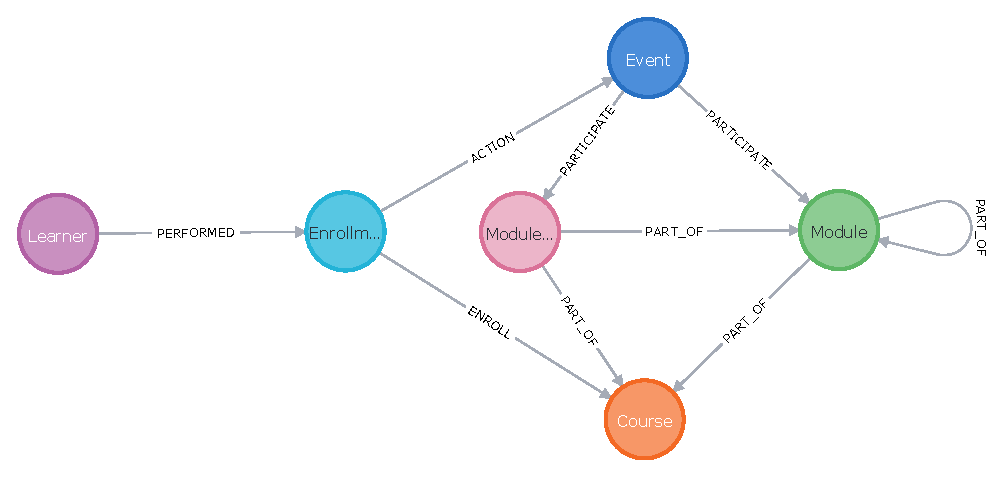
\includegraphics[width=0.45\textwidth]{assets/graph-modeling}
        }
        \caption{แบบจำลองความสัมพันธ์ของกราฟในฐานข้อมูล}
        \label{fig:graph-modeling}
    \end{figure}

    ซึ่งจากการเรียกดูข้อมูลพบว่า มีโหนดในฐานข้อมูลทั้งสิ้นรวม 5,434,977 โหนด โดยแบ่งออกเป็น 
    % MATCH (n) 
    % RETURN DISTINCT count(labels(n)) AS node_count, labels(n)[0] AS node_name;
    \begin{table}[ht!]
        \caption[nodecountinfo]{จำนวนโหนดในฐานข้อมูลแบ่งตามประเภท}
        \label{tab:node-details}
        \begin{tabular}{p{3cm} p{5cm}}
            \hline
            \thead{ป้ายกำกับโหนด}   & \thead{จำนวนโหนด (โหนด)} \\
            \hline
            \textit{Course}         & 39 \\
            \textit{Enrollment}     & 72,395 \\
            \textit{Learner}        & 53,870 \\
            \textit{Module}         & 26,750 \\
            \textit{ModuleObject}   & 26,032 \\
            \textit{Event}          & 5,255,891 \\
            \hline
        \end{tabular}
    \end{table}

    % MATCH (e:Enrollment {learning_status: "dropout"})
    % RETURN COUNT(e) AS total_dropout;
    โดยสิ่งที่น่าสนใจคือ จากจำนวนผู้เรียนที่ลงทะเบียนเรียนทั้งสิ้น 72,395 ครั้ง 
    ดังที่แสดงไว้ในตารางที่ \ref{tab:node-details} แล้วนั้น พบว่าเกิด{\dropout}ไปทั้งสิ้น
    57,366 รายการ หรือคิดเป็น 79.24\% ของข้อมูลการลงทะเบียนในชุดข้อมูลนี้

    \section[result]{ผลลัพธ์การดำเนินงาน}
    lorem ipsum

    \section[conclusions]{สรุปผลการศึกษา}
    lorem ipsum

    \bibliographystyle{IEEEtran}
    \bibliography{sna-ref}
\end{document}